\documentclass{standalone}
\usepackage{tikz}
\usetikzlibrary{patterns, positioning}


\begin{document}
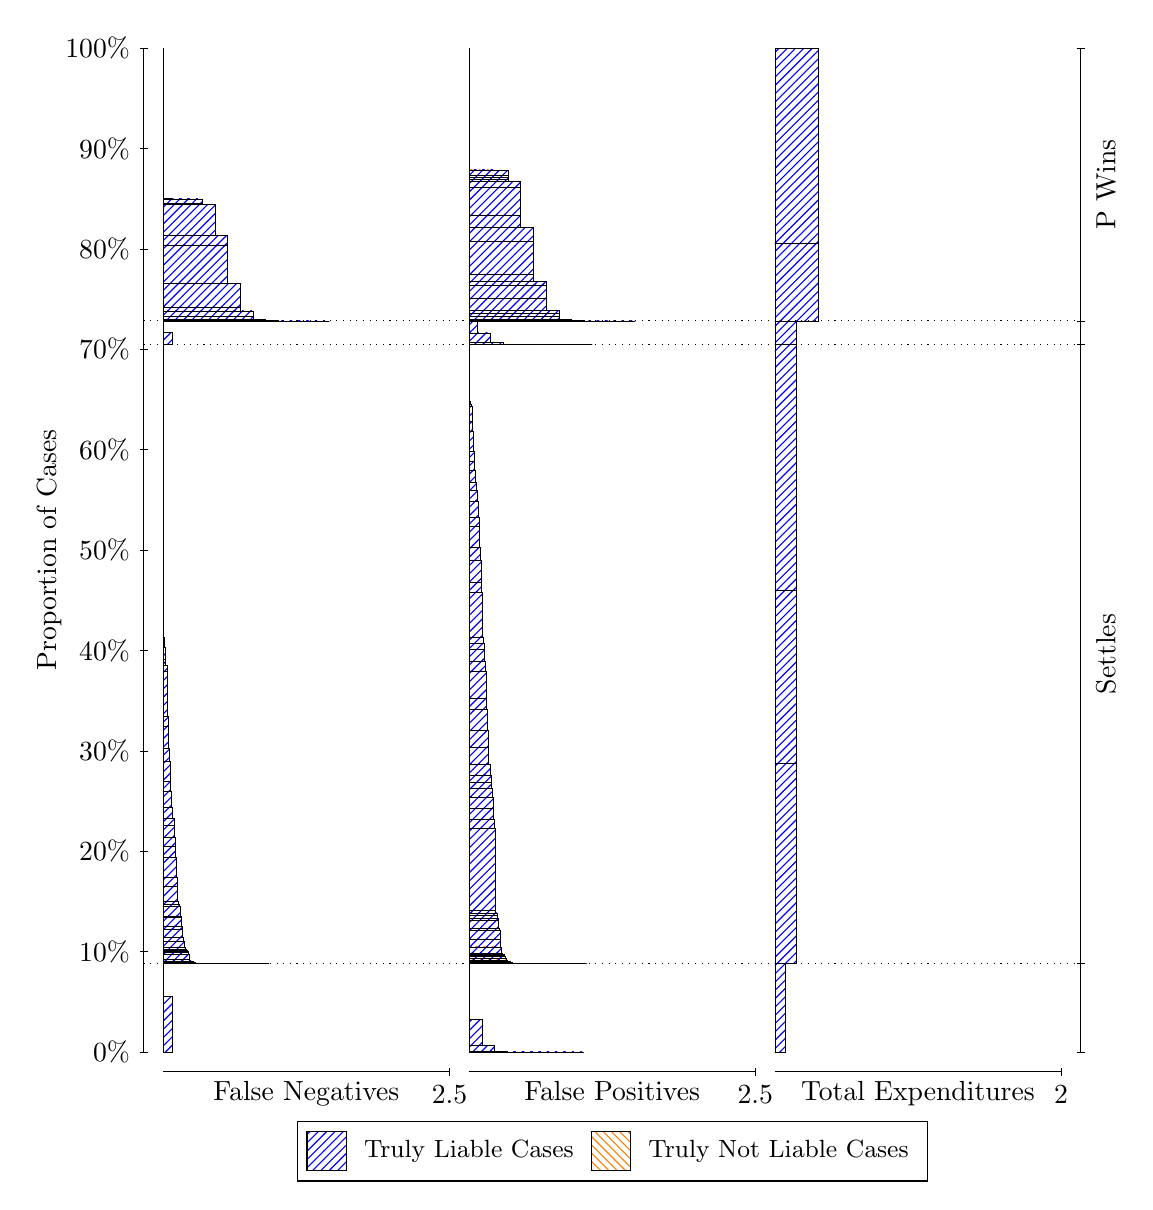
\begin{tikzpicture}
\draw[black, very thin] (1.5,1.75) -- (1.5,14.5);
\node[rotate=90, text=black, anchor=center] at (0.3, 8.125) {Proportion of Cases};
\draw[black, very thin] (1.45,1.75) -- (1.55,1.75);
\node[text=black, anchor=east] at (1.45, 1.75) {0\%};
\draw[black, very thin] (1.45,3.025) -- (1.55,3.025);
\node[text=black, anchor=east] at (1.45, 3.025) {10\%};
\draw[black, very thin] (1.45,4.3) -- (1.55,4.3);
\node[text=black, anchor=east] at (1.45, 4.3) {20\%};
\draw[black, very thin] (1.45,5.575) -- (1.55,5.575);
\node[text=black, anchor=east] at (1.45, 5.575) {30\%};
\draw[black, very thin] (1.45,6.85) -- (1.55,6.85);
\node[text=black, anchor=east] at (1.45, 6.85) {40\%};
\draw[black, very thin] (1.45,8.125) -- (1.55,8.125);
\node[text=black, anchor=east] at (1.45, 8.125) {50\%};
\draw[black, very thin] (1.45,9.4) -- (1.55,9.4);
\node[text=black, anchor=east] at (1.45, 9.4) {60\%};
\draw[black, very thin] (1.45,10.675) -- (1.55,10.675);
\node[text=black, anchor=east] at (1.45, 10.675) {70\%};
\draw[black, very thin] (1.45,11.95) -- (1.55,11.95);
\node[text=black, anchor=east] at (1.45, 11.95) {80\%};
\draw[black, very thin] (1.45,13.225) -- (1.55,13.225);
\node[text=black, anchor=east] at (1.45, 13.225) {90\%};
\draw[black, very thin] (1.45,14.5) -- (1.55,14.5);
\node[text=black, anchor=east] at (1.45, 14.5) {100\%};

\draw[black, very thin] (13.4,1.75) -- (13.4,14.5);
\draw[black, very thin] (13.35,1.75) -- (13.45,1.75);
\node[anchor=west] at (13.35, 1.75) {};
\draw[black, very thin] (13.35,2.8721) -- (13.45,2.8721);
\node[anchor=west] at (13.35, 2.8721) {};
\draw[black, very thin] (13.35,10.734) -- (13.45,10.734);
\node[anchor=west] at (13.35, 10.734) {};
\draw[black, very thin] (13.35,11.036) -- (13.45,11.036);
\node[anchor=west] at (13.35, 11.036) {};
\draw[black, very thin] (13.35,14.5) -- (13.45,14.5);
\node[anchor=west] at (13.35, 14.5) {};

\draw[black, very thin, pattern color=blue, pattern=north east lines] (1.75,1.75) rectangle (1.859,2.4561);
\draw[black, very thin, pattern color=orange, pattern=north west lines] (1.75,2.4561) rectangle (1.75,2.4561);
\draw[black, very thin, pattern color=blue, pattern=north east lines] (1.75,2.4561) rectangle (1.75,2.8721);
\draw[black, very thin, pattern color=blue, pattern=north east lines] (1.75,2.8721) rectangle (3.0943,2.8721);
\draw[black, very thin, pattern color=blue, pattern=north east lines] (1.75,2.8721) rectangle (3.0217,2.8721);
\draw[black, very thin, pattern color=blue, pattern=north east lines] (1.75,2.8721) rectangle (2.949,2.8721);
\draw[black, very thin, pattern color=blue, pattern=north east lines] (1.75,2.8721) rectangle (2.9329,2.8721);
\draw[black, very thin, pattern color=blue, pattern=north east lines] (1.75,2.8721) rectangle (2.8763,2.8721);
\draw[black, very thin, pattern color=blue, pattern=north east lines] (1.75,2.8721) rectangle (2.8602,2.8721);
\draw[black, very thin, pattern color=blue, pattern=north east lines] (1.75,2.8721) rectangle (2.8037,2.8721);
\draw[black, very thin, pattern color=blue, pattern=north east lines] (1.75,2.8721) rectangle (2.7875,2.8721);
\draw[black, very thin, pattern color=blue, pattern=north east lines] (1.75,2.8721) rectangle (2.7714,2.8721);
\draw[black, very thin, pattern color=blue, pattern=north east lines] (1.75,2.8721) rectangle (2.731,2.8721);
\draw[black, very thin, pattern color=blue, pattern=north east lines] (1.75,2.8721) rectangle (2.7149,2.8721);
\draw[black, very thin, pattern color=blue, pattern=north east lines] (1.75,2.8721) rectangle (2.6987,2.8721);
\draw[black, very thin, pattern color=blue, pattern=north east lines] (1.75,2.8721) rectangle (2.6583,2.8721);
\draw[black, very thin, pattern color=blue, pattern=north east lines] (1.75,2.8721) rectangle (2.6422,2.8721);
\draw[black, very thin, pattern color=blue, pattern=north east lines] (1.75,2.8721) rectangle (2.626,2.8721);
\draw[black, very thin, pattern color=blue, pattern=north east lines] (1.75,2.8721) rectangle (2.6099,2.8721);
\draw[black, very thin, pattern color=blue, pattern=north east lines] (1.75,2.8721) rectangle (2.5857,2.8721);
\draw[black, very thin, pattern color=blue, pattern=north east lines] (1.75,2.8721) rectangle (2.5695,2.8721);
\draw[black, very thin, pattern color=blue, pattern=north east lines] (1.75,2.8721) rectangle (2.5534,2.8721);
\draw[black, very thin, pattern color=blue, pattern=north east lines] (1.75,2.8721) rectangle (2.5372,2.8721);
\draw[black, very thin, pattern color=blue, pattern=north east lines] (1.75,2.8721) rectangle (2.513,2.8721);
\draw[black, very thin, pattern color=blue, pattern=north east lines] (1.75,2.8721) rectangle (2.4969,2.8721);
\draw[black, very thin, pattern color=blue, pattern=north east lines] (1.75,2.8721) rectangle (2.4807,2.8721);
\draw[black, very thin, pattern color=blue, pattern=north east lines] (1.75,2.8721) rectangle (2.4646,2.8721);
\draw[black, very thin, pattern color=blue, pattern=north east lines] (1.75,2.8721) rectangle (2.4484,2.8721);
\draw[black, very thin, pattern color=blue, pattern=north east lines] (1.75,2.8721) rectangle (2.4403,2.8721);
\draw[black, very thin, pattern color=blue, pattern=north east lines] (1.75,2.8721) rectangle (2.4242,2.8721);
\draw[black, very thin, pattern color=blue, pattern=north east lines] (1.75,2.8721) rectangle (2.408,2.8721);
\draw[black, very thin, pattern color=blue, pattern=north east lines] (1.75,2.8721) rectangle (2.3919,2.8721);
\draw[black, very thin, pattern color=blue, pattern=north east lines] (1.75,2.8721) rectangle (2.3757,2.8721);
\draw[black, very thin, pattern color=blue, pattern=north east lines] (1.75,2.8721) rectangle (2.3677,2.8721);
\draw[black, very thin, pattern color=blue, pattern=north east lines] (1.75,2.8721) rectangle (2.3677,2.8721);
\draw[black, very thin, pattern color=blue, pattern=north east lines] (1.75,2.8721) rectangle (2.3515,2.8721);
\draw[black, very thin, pattern color=blue, pattern=north east lines] (1.75,2.8721) rectangle (2.3354,2.8721);
\draw[black, very thin, pattern color=blue, pattern=north east lines] (1.75,2.8721) rectangle (2.3192,2.8722);
\draw[black, very thin, pattern color=blue, pattern=north east lines] (1.75,2.8722) rectangle (2.3031,2.8723);
\draw[black, very thin, pattern color=blue, pattern=north east lines] (1.75,2.8723) rectangle (2.295,2.8723);
\draw[black, very thin, pattern color=blue, pattern=north east lines] (1.75,2.8723) rectangle (2.2869,2.8723);
\draw[black, very thin, pattern color=blue, pattern=north east lines] (1.75,2.8723) rectangle (2.2789,2.8723);
\draw[black, very thin, pattern color=blue, pattern=north east lines] (1.75,2.8723) rectangle (2.2627,2.8724);
\draw[black, very thin, pattern color=blue, pattern=north east lines] (1.75,2.8724) rectangle (2.2466,2.8728);
\draw[black, very thin, pattern color=blue, pattern=north east lines] (1.75,2.8728) rectangle (2.2304,2.8734);
\draw[black, very thin, pattern color=blue, pattern=north east lines] (1.75,2.8734) rectangle (2.2223,2.8735);
\draw[black, very thin, pattern color=blue, pattern=north east lines] (1.75,2.8735) rectangle (2.2143,2.874);
\draw[black, very thin, pattern color=blue, pattern=north east lines] (1.75,2.874) rectangle (2.2062,2.874);
\draw[black, very thin, pattern color=blue, pattern=north east lines] (1.75,2.874) rectangle (2.2062,2.8742);
\draw[black, very thin, pattern color=blue, pattern=north east lines] (1.75,2.8742) rectangle (2.19,2.8748);
\draw[black, very thin, pattern color=blue, pattern=north east lines] (1.75,2.8748) rectangle (2.1739,2.8795);
\draw[black, very thin, pattern color=blue, pattern=north east lines] (1.75,2.8795) rectangle (2.1577,2.886);
\draw[black, very thin, pattern color=blue, pattern=north east lines] (1.75,2.886) rectangle (2.1497,2.8888);
\draw[black, very thin, pattern color=blue, pattern=north east lines] (1.75,2.8888) rectangle (2.1416,2.8954);
\draw[black, very thin, pattern color=blue, pattern=north east lines] (1.75,2.8954) rectangle (2.1335,2.896);
\draw[black, very thin, pattern color=blue, pattern=north east lines] (1.75,2.896) rectangle (2.1254,2.9016);
\draw[black, very thin, pattern color=blue, pattern=north east lines] (1.75,2.9016) rectangle (2.1174,2.9037);
\draw[black, very thin, pattern color=blue, pattern=north east lines] (1.75,2.9037) rectangle (2.1012,2.9056);
\draw[black, very thin, pattern color=blue, pattern=north east lines] (1.75,2.9056) rectangle (2.0851,2.9244);
\draw[black, very thin, pattern color=blue, pattern=north east lines] (1.75,2.9244) rectangle (2.077,2.9944);
\draw[black, very thin, pattern color=blue, pattern=north east lines] (1.75,2.9944) rectangle (2.0689,3.0161);
\draw[black, very thin, pattern color=blue, pattern=north east lines] (1.75,3.0161) rectangle (2.0609,3.0251);
\draw[black, very thin, pattern color=blue, pattern=north east lines] (1.75,3.0251) rectangle (2.0528,3.0456);
\draw[black, very thin, pattern color=blue, pattern=north east lines] (1.75,3.0456) rectangle (2.0447,3.0457);
\draw[black, very thin, pattern color=blue, pattern=north east lines] (1.75,3.0457) rectangle (2.0447,3.0542);
\draw[black, very thin, pattern color=blue, pattern=north east lines] (1.75,3.0542) rectangle (2.0286,3.0759);
\draw[black, very thin, pattern color=blue, pattern=north east lines] (1.75,3.0759) rectangle (2.0124,3.1534);
\draw[black, very thin, pattern color=blue, pattern=north east lines] (1.75,3.1534) rectangle (2.0043,3.208);
\draw[black, very thin, pattern color=blue, pattern=north east lines] (1.75,3.208) rectangle (1.9963,3.3121);
\draw[black, very thin, pattern color=blue, pattern=north east lines] (1.75,3.3121) rectangle (1.9882,3.3504);
\draw[black, very thin, pattern color=blue, pattern=north east lines] (1.75,3.3504) rectangle (1.9801,3.4575);
\draw[black, very thin, pattern color=blue, pattern=north east lines] (1.75,3.4575) rectangle (1.972,3.4774);
\draw[black, very thin, pattern color=blue, pattern=north east lines] (1.75,3.4774) rectangle (1.964,3.5954);
\draw[black, very thin, pattern color=blue, pattern=north east lines] (1.75,3.5954) rectangle (1.9559,3.6271);
\draw[black, very thin, pattern color=blue, pattern=north east lines] (1.75,3.6271) rectangle (1.9397,3.6585);
\draw[black, very thin, pattern color=blue, pattern=north east lines] (1.75,3.6585) rectangle (1.9317,3.8502);
\draw[black, very thin, pattern color=blue, pattern=north east lines] (1.75,3.8502) rectangle (1.9236,3.9701);
\draw[black, very thin, pattern color=blue, pattern=north east lines] (1.75,3.9701) rectangle (1.9155,4.2217);
\draw[black, very thin, pattern color=blue, pattern=north east lines] (1.75,4.2217) rectangle (1.9074,4.3603);
\draw[black, very thin, pattern color=blue, pattern=north east lines] (1.75,4.3603) rectangle (1.8994,4.4741);
\draw[black, very thin, pattern color=blue, pattern=north east lines] (1.75,4.4741) rectangle (1.8913,4.6235);
\draw[black, very thin, pattern color=blue, pattern=north east lines] (1.75,4.6235) rectangle (1.8832,4.6238);
\draw[black, very thin, pattern color=blue, pattern=north east lines] (1.75,4.6238) rectangle (1.8832,4.7191);
\draw[black, very thin, pattern color=blue, pattern=north east lines] (1.75,4.7191) rectangle (1.8671,4.8563);
\draw[black, very thin, pattern color=blue, pattern=north east lines] (1.75,4.8563) rectangle (1.8509,5.0624);
\draw[black, very thin, pattern color=blue, pattern=north east lines] (1.75,5.0624) rectangle (1.8429,5.1831);
\draw[black, very thin, pattern color=blue, pattern=north east lines] (1.75,5.1831) rectangle (1.8348,5.4447);
\draw[black, very thin, pattern color=blue, pattern=north east lines] (1.75,5.4447) rectangle (1.8267,5.6082);
\draw[black, very thin, pattern color=blue, pattern=north east lines] (1.75,5.6082) rectangle (1.8186,5.8918);
\draw[black, very thin, pattern color=blue, pattern=north east lines] (1.75,5.8918) rectangle (1.8106,6.0125);
\draw[black, very thin, pattern color=blue, pattern=north east lines] (1.75,6.0125) rectangle (1.8025,6.5838);
\draw[black, very thin, pattern color=blue, pattern=north east lines] (1.75,6.5838) rectangle (1.7944,6.6632);
\draw[black, very thin, pattern color=blue, pattern=north east lines] (1.75,6.6632) rectangle (1.7783,6.7424);
\draw[black, very thin, pattern color=blue, pattern=north east lines] (1.75,6.7424) rectangle (1.7702,6.8924);
\draw[black, very thin, pattern color=blue, pattern=north east lines] (1.75,6.8924) rectangle (1.7621,7.0157);
\draw[black, very thin, pattern color=blue, pattern=north east lines] (1.75,7.0157) rectangle (1.754,7.3577);
\draw[black, very thin, pattern color=orange, pattern=north west lines] (1.75,7.3577) rectangle (1.75,7.3577);
\draw[black, very thin, pattern color=blue, pattern=north east lines] (1.75,7.3577) rectangle (1.75,10.734);
\draw[black, very thin, pattern color=blue, pattern=north east lines] (1.75,10.734) rectangle (1.859,10.886);
\draw[black, very thin, pattern color=orange, pattern=north west lines] (1.75,10.886) rectangle (1.75,10.886);
\draw[black, very thin, pattern color=blue, pattern=north east lines] (1.75,10.886) rectangle (1.75,11.036);
\draw[black, very thin, pattern color=blue, pattern=north east lines] (1.75,11.036) rectangle (3.8573,11.036);
\draw[black, very thin, pattern color=blue, pattern=north east lines] (1.75,11.036) rectangle (3.6959,11.036);
\draw[black, very thin, pattern color=blue, pattern=north east lines] (1.75,11.036) rectangle (3.5344,11.036);
\draw[black, very thin, pattern color=blue, pattern=north east lines] (1.75,11.036) rectangle (3.5344,11.036);
\draw[black, very thin, pattern color=blue, pattern=north east lines] (1.75,11.036) rectangle (3.3729,11.036);
\draw[black, very thin, pattern color=blue, pattern=north east lines] (1.75,11.036) rectangle (3.2114,11.038);
\draw[black, very thin, pattern color=blue, pattern=north east lines] (1.75,11.038) rectangle (3.0499,11.057);
\draw[black, very thin, pattern color=blue, pattern=north east lines] (1.75,11.057) rectangle (2.8884,11.096);
\draw[black, very thin, pattern color=blue, pattern=north east lines] (1.75,11.096) rectangle (2.8884,11.161);
\draw[black, very thin, pattern color=blue, pattern=north east lines] (1.75,11.161) rectangle (2.727,11.212);
\draw[black, very thin, pattern color=blue, pattern=north east lines] (1.75,11.212) rectangle (2.727,11.51);
\draw[black, very thin, pattern color=blue, pattern=north east lines] (1.75,11.51) rectangle (2.6624,11.51);
\draw[black, very thin, pattern color=blue, pattern=north east lines] (1.75,11.51) rectangle (2.5655,11.999);
\draw[black, very thin, pattern color=blue, pattern=north east lines] (1.75,11.999) rectangle (2.5655,12.122);
\draw[black, very thin, pattern color=blue, pattern=north east lines] (1.75,12.122) rectangle (2.5009,12.122);
\draw[black, very thin, pattern color=blue, pattern=north east lines] (1.75,12.122) rectangle (2.5009,12.122);
\draw[black, very thin, pattern color=blue, pattern=north east lines] (1.75,12.122) rectangle (2.404,12.518);
\draw[black, very thin, pattern color=blue, pattern=north east lines] (1.75,12.518) rectangle (2.3394,12.518);
\draw[black, very thin, pattern color=blue, pattern=north east lines] (1.75,12.518) rectangle (2.2425,12.523);
\draw[black, very thin, pattern color=blue, pattern=north east lines] (1.75,12.523) rectangle (2.2425,12.576);
\draw[black, very thin, pattern color=blue, pattern=north east lines] (1.75,12.576) rectangle (2.2425,12.583);
\draw[black, very thin, pattern color=blue, pattern=north east lines] (1.75,12.583) rectangle (2.1779,12.583);
\draw[black, very thin, pattern color=blue, pattern=north east lines] (1.75,12.583) rectangle (2.1779,12.583);
\draw[black, very thin, pattern color=blue, pattern=north east lines] (1.75,12.583) rectangle (2.081,12.583);
\draw[black, very thin, pattern color=blue, pattern=north east lines] (1.75,12.583) rectangle (2.081,12.583);
\draw[black, very thin, pattern color=blue, pattern=north east lines] (1.75,12.583) rectangle (2.0164,12.583);
\draw[black, very thin, pattern color=blue, pattern=north east lines] (1.75,12.583) rectangle (2.0164,12.583);
\draw[black, very thin, pattern color=blue, pattern=north east lines] (1.75,12.583) rectangle (1.9196,12.583);
\draw[black, very thin, pattern color=blue, pattern=north east lines] (1.75,12.583) rectangle (1.9196,12.583);
\draw[black, very thin, pattern color=blue, pattern=north east lines] (1.75,12.583) rectangle (1.855,12.584);
\draw[black, very thin, pattern color=blue, pattern=north east lines] (1.75,12.584) rectangle (1.855,12.59);
\draw[black, very thin, pattern color=blue, pattern=north east lines] (1.75,12.59) rectangle (1.7581,12.59);
\draw[black, very thin, pattern color=blue, pattern=north east lines] (1.75,12.59) rectangle (1.7581,12.59);
\draw[black, very thin, pattern color=orange, pattern=north west lines] (1.75,12.59) rectangle (1.75,12.59);
\draw[black, very thin, pattern color=blue, pattern=north east lines] (1.75,12.59) rectangle (1.75,14.5);
\draw[black, very thin, pattern color=orange, pattern=north west lines] (5.6333,1.75) rectangle (7.0867,1.75);
\draw[black, very thin, pattern color=blue, pattern=north east lines] (5.6333,1.75) rectangle (7.0867,1.75);
\draw[black, very thin, pattern color=blue, pattern=north east lines] (5.6333,1.75) rectangle (6.9252,1.75);
\draw[black, very thin, pattern color=blue, pattern=north east lines] (5.6333,1.75) rectangle (6.7637,1.75);
\draw[black, very thin, pattern color=blue, pattern=north east lines] (5.6333,1.75) rectangle (6.6022,1.75);
\draw[black, very thin, pattern color=blue, pattern=north east lines] (5.6333,1.75) rectangle (6.4407,1.75);
\draw[black, very thin, pattern color=blue, pattern=north east lines] (5.6333,1.75) rectangle (6.2793,1.7503);
\draw[black, very thin, pattern color=blue, pattern=north east lines] (5.6333,1.7503) rectangle (6.1178,1.7579);
\draw[black, very thin, pattern color=blue, pattern=north east lines] (5.6333,1.7579) rectangle (5.9563,1.8357);
\draw[black, very thin, pattern color=blue, pattern=north east lines] (5.6333,1.8357) rectangle (5.7948,2.166);
\draw[black, very thin, pattern color=blue, pattern=north east lines] (5.6333,2.166) rectangle (5.6333,2.8721);
\draw[black, very thin, pattern color=orange, pattern=north west lines] (5.6333,2.8721) rectangle (7.123,2.8721);
\draw[black, very thin, pattern color=blue, pattern=north east lines] (5.6333,2.8721) rectangle (7.123,2.8721);
\draw[black, very thin, pattern color=orange, pattern=north west lines] (5.6333,2.8721) rectangle (7.0503,2.8721);
\draw[black, very thin, pattern color=blue, pattern=north east lines] (5.6333,2.8721) rectangle (7.0503,2.8721);
\draw[black, very thin, pattern color=orange, pattern=north west lines] (5.6333,2.8721) rectangle (6.9777,2.8721);
\draw[black, very thin, pattern color=blue, pattern=north east lines] (5.6333,2.8721) rectangle (6.9777,2.8721);
\draw[black, very thin, pattern color=blue, pattern=north east lines] (5.6333,2.8721) rectangle (6.9615,2.8721);
\draw[black, very thin, pattern color=orange, pattern=north west lines] (5.6333,2.8721) rectangle (6.905,2.8721);
\draw[black, very thin, pattern color=blue, pattern=north east lines] (5.6333,2.8721) rectangle (6.905,2.8721);
\draw[black, very thin, pattern color=blue, pattern=north east lines] (5.6333,2.8721) rectangle (6.8889,2.8721);
\draw[black, very thin, pattern color=orange, pattern=north west lines] (5.6333,2.8721) rectangle (6.8323,2.8721);
\draw[black, very thin, pattern color=blue, pattern=north east lines] (5.6333,2.8721) rectangle (6.8323,2.8721);
\draw[black, very thin, pattern color=blue, pattern=north east lines] (5.6333,2.8721) rectangle (6.8162,2.8721);
\draw[black, very thin, pattern color=blue, pattern=north east lines] (5.6333,2.8721) rectangle (6.8,2.8721);
\draw[black, very thin, pattern color=orange, pattern=north west lines] (5.6333,2.8721) rectangle (6.7597,2.8721);
\draw[black, very thin, pattern color=blue, pattern=north east lines] (5.6333,2.8721) rectangle (6.7597,2.8721);
\draw[black, very thin, pattern color=blue, pattern=north east lines] (5.6333,2.8721) rectangle (6.7435,2.8721);
\draw[black, very thin, pattern color=blue, pattern=north east lines] (5.6333,2.8721) rectangle (6.7274,2.8721);
\draw[black, very thin, pattern color=orange, pattern=north west lines] (5.6333,2.8721) rectangle (6.687,2.8721);
\draw[black, very thin, pattern color=blue, pattern=north east lines] (5.6333,2.8721) rectangle (6.687,2.8721);
\draw[black, very thin, pattern color=orange, pattern=north west lines] (5.6333,2.8721) rectangle (6.687,2.8721);
\draw[black, very thin, pattern color=blue, pattern=north east lines] (5.6333,2.8721) rectangle (6.687,2.8721);
\draw[black, very thin, pattern color=blue, pattern=north east lines] (5.6333,2.8721) rectangle (6.6709,2.8721);
\draw[black, very thin, pattern color=blue, pattern=north east lines] (5.6333,2.8721) rectangle (6.6547,2.8721);
\draw[black, very thin, pattern color=blue, pattern=north east lines] (5.6333,2.8721) rectangle (6.6386,2.8721);
\draw[black, very thin, pattern color=orange, pattern=north west lines] (5.6333,2.8721) rectangle (6.6143,2.8721);
\draw[black, very thin, pattern color=blue, pattern=north east lines] (5.6333,2.8721) rectangle (6.6143,2.8721);
\draw[black, very thin, pattern color=blue, pattern=north east lines] (5.6333,2.8721) rectangle (6.5982,2.8721);
\draw[black, very thin, pattern color=blue, pattern=north east lines] (5.6333,2.8721) rectangle (6.582,2.8721);
\draw[black, very thin, pattern color=blue, pattern=north east lines] (5.6333,2.8721) rectangle (6.5659,2.8721);
\draw[black, very thin, pattern color=orange, pattern=north west lines] (5.6333,2.8721) rectangle (6.5417,2.8721);
\draw[black, very thin, pattern color=blue, pattern=north east lines] (5.6333,2.8721) rectangle (6.5417,2.8721);
\draw[black, very thin, pattern color=blue, pattern=north east lines] (5.6333,2.8721) rectangle (6.5255,2.8721);
\draw[black, very thin, pattern color=blue, pattern=north east lines] (5.6333,2.8721) rectangle (6.5255,2.8721);
\draw[black, very thin, pattern color=blue, pattern=north east lines] (5.6333,2.8721) rectangle (6.5094,2.8721);
\draw[black, very thin, pattern color=blue, pattern=north east lines] (5.6333,2.8721) rectangle (6.4932,2.8721);
\draw[black, very thin, pattern color=blue, pattern=north east lines] (5.6333,2.8721) rectangle (6.4771,2.8721);
\draw[black, very thin, pattern color=orange, pattern=north west lines] (5.6333,2.8721) rectangle (6.469,2.8721);
\draw[black, very thin, pattern color=blue, pattern=north east lines] (5.6333,2.8721) rectangle (6.469,2.8721);
\draw[black, very thin, pattern color=blue, pattern=north east lines] (5.6333,2.8721) rectangle (6.4529,2.8721);
\draw[black, very thin, pattern color=blue, pattern=north east lines] (5.6333,2.8721) rectangle (6.4367,2.8721);
\draw[black, very thin, pattern color=blue, pattern=north east lines] (5.6333,2.8721) rectangle (6.4206,2.8721);
\draw[black, very thin, pattern color=blue, pattern=north east lines] (5.6333,2.8721) rectangle (6.4044,2.8721);
\draw[black, very thin, pattern color=orange, pattern=north west lines] (5.6333,2.8721) rectangle (6.3963,2.8721);
\draw[black, very thin, pattern color=blue, pattern=north east lines] (5.6333,2.8721) rectangle (6.3963,2.8721);
\draw[black, very thin, pattern color=blue, pattern=north east lines] (5.6333,2.8721) rectangle (6.3802,2.8721);
\draw[black, very thin, pattern color=blue, pattern=north east lines] (5.6333,2.8721) rectangle (6.364,2.8721);
\draw[black, very thin, pattern color=blue, pattern=north east lines] (5.6333,2.8721) rectangle (6.364,2.8721);
\draw[black, very thin, pattern color=blue, pattern=north east lines] (5.6333,2.8721) rectangle (6.3479,2.8722);
\draw[black, very thin, pattern color=blue, pattern=north east lines] (5.6333,2.8722) rectangle (6.3317,2.8722);
\draw[black, very thin, pattern color=orange, pattern=north west lines] (5.6333,2.8722) rectangle (6.3237,2.8722);
\draw[black, very thin, pattern color=blue, pattern=north east lines] (5.6333,2.8722) rectangle (6.3237,2.8723);
\draw[black, very thin, pattern color=blue, pattern=north east lines] (5.6333,2.8723) rectangle (6.3156,2.8723);
\draw[black, very thin, pattern color=blue, pattern=north east lines] (5.6333,2.8723) rectangle (6.3075,2.8723);
\draw[black, very thin, pattern color=blue, pattern=north east lines] (5.6333,2.8723) rectangle (6.2914,2.8723);
\draw[black, very thin, pattern color=blue, pattern=north east lines] (5.6333,2.8723) rectangle (6.2752,2.8728);
\draw[black, very thin, pattern color=blue, pattern=north east lines] (5.6333,2.8728) rectangle (6.2591,2.8733);
\draw[black, very thin, pattern color=orange, pattern=north west lines] (5.6333,2.8733) rectangle (6.251,2.8733);
\draw[black, very thin, pattern color=blue, pattern=north east lines] (5.6333,2.8733) rectangle (6.251,2.8734);
\draw[black, very thin, pattern color=blue, pattern=north east lines] (5.6333,2.8734) rectangle (6.2429,2.8737);
\draw[black, very thin, pattern color=blue, pattern=north east lines] (5.6333,2.8737) rectangle (6.2349,2.8738);
\draw[black, very thin, pattern color=blue, pattern=north east lines] (5.6333,2.8738) rectangle (6.2187,2.8744);
\draw[black, very thin, pattern color=blue, pattern=north east lines] (5.6333,2.8744) rectangle (6.2026,2.8791);
\draw[black, very thin, pattern color=blue, pattern=north east lines] (5.6333,2.8791) rectangle (6.2026,2.8791);
\draw[black, very thin, pattern color=blue, pattern=north east lines] (5.6333,2.8791) rectangle (6.1864,2.8857);
\draw[black, very thin, pattern color=orange, pattern=north west lines] (5.6333,2.8857) rectangle (6.1783,2.8857);
\draw[black, very thin, pattern color=blue, pattern=north east lines] (5.6333,2.8857) rectangle (6.1783,2.887);
\draw[black, very thin, pattern color=blue, pattern=north east lines] (5.6333,2.887) rectangle (6.1703,2.8931);
\draw[black, very thin, pattern color=blue, pattern=north east lines] (5.6333,2.8931) rectangle (6.1622,2.8939);
\draw[black, very thin, pattern color=blue, pattern=north east lines] (5.6333,2.8939) rectangle (6.1541,2.8957);
\draw[black, very thin, pattern color=blue, pattern=north east lines] (5.6333,2.8957) rectangle (6.146,2.8977);
\draw[black, very thin, pattern color=blue, pattern=north east lines] (5.6333,2.8977) rectangle (6.1299,2.8997);
\draw[black, very thin, pattern color=blue, pattern=north east lines] (5.6333,2.8997) rectangle (6.1137,2.9184);
\draw[black, very thin, pattern color=orange, pattern=north west lines] (5.6333,2.9184) rectangle (6.1057,2.9184);
\draw[black, very thin, pattern color=blue, pattern=north east lines] (5.6333,2.9184) rectangle (6.1057,2.9382);
\draw[black, very thin, pattern color=blue, pattern=north east lines] (5.6333,2.9382) rectangle (6.0976,2.9593);
\draw[black, very thin, pattern color=blue, pattern=north east lines] (5.6333,2.9593) rectangle (6.0895,2.9668);
\draw[black, very thin, pattern color=blue, pattern=north east lines] (5.6333,2.9668) rectangle (6.0814,2.9782);
\draw[black, very thin, pattern color=blue, pattern=north east lines] (5.6333,2.9782) rectangle (6.0734,2.986);
\draw[black, very thin, pattern color=blue, pattern=north east lines] (5.6333,2.986) rectangle (6.0572,3.0076);
\draw[black, very thin, pattern color=blue, pattern=north east lines] (5.6333,3.0076) rectangle (6.0411,3.0851);
\draw[black, very thin, pattern color=blue, pattern=north east lines] (5.6333,3.0851) rectangle (6.0411,3.0851);
\draw[black, very thin, pattern color=orange, pattern=north west lines] (5.6333,3.0851) rectangle (6.033,3.0851);
\draw[black, very thin, pattern color=blue, pattern=north east lines] (5.6333,3.0851) rectangle (6.033,3.1861);
\draw[black, very thin, pattern color=blue, pattern=north east lines] (5.6333,3.1861) rectangle (6.0249,3.2915);
\draw[black, very thin, pattern color=blue, pattern=north east lines] (5.6333,3.2915) rectangle (6.0169,3.3184);
\draw[black, very thin, pattern color=blue, pattern=north east lines] (5.6333,3.3184) rectangle (6.0088,3.4255);
\draw[black, very thin, pattern color=blue, pattern=north east lines] (5.6333,3.4255) rectangle (6.0007,3.4468);
\draw[black, very thin, pattern color=blue, pattern=north east lines] (5.6333,3.4468) rectangle (5.9926,3.4835);
\draw[black, very thin, pattern color=blue, pattern=north east lines] (5.6333,3.4835) rectangle (5.9846,3.515);
\draw[black, very thin, pattern color=blue, pattern=north east lines] (5.6333,3.515) rectangle (5.9684,3.5464);
\draw[black, very thin, pattern color=orange, pattern=north west lines] (5.6333,3.5464) rectangle (5.9603,3.5464);
\draw[black, very thin, pattern color=blue, pattern=north east lines] (5.6333,3.5464) rectangle (5.9603,4.5869);
\draw[black, very thin, pattern color=blue, pattern=north east lines] (5.6333,4.5869) rectangle (5.9523,4.706);
\draw[black, very thin, pattern color=blue, pattern=north east lines] (5.6333,4.706) rectangle (5.9442,4.847);
\draw[black, very thin, pattern color=blue, pattern=north east lines] (5.6333,4.847) rectangle (5.9361,4.9885);
\draw[black, very thin, pattern color=blue, pattern=north east lines] (5.6333,4.9885) rectangle (5.928,5.0939);
\draw[black, very thin, pattern color=blue, pattern=north east lines] (5.6333,5.0939) rectangle (5.92,5.1765);
\draw[black, very thin, pattern color=blue, pattern=north east lines] (5.6333,5.1765) rectangle (5.9119,5.2702);
\draw[black, very thin, pattern color=blue, pattern=north east lines] (5.6333,5.2702) rectangle (5.8957,5.4074);
\draw[black, very thin, pattern color=blue, pattern=north east lines] (5.6333,5.4074) rectangle (5.8796,5.6138);
\draw[black, very thin, pattern color=blue, pattern=north east lines] (5.6333,5.6138) rectangle (5.8796,5.614);
\draw[black, very thin, pattern color=blue, pattern=north east lines] (5.6333,5.614) rectangle (5.8715,5.8351);
\draw[black, very thin, pattern color=blue, pattern=north east lines] (5.6333,5.8351) rectangle (5.8634,6.105);
\draw[black, very thin, pattern color=blue, pattern=north east lines] (5.6333,6.105) rectangle (5.8554,6.2481);
\draw[black, very thin, pattern color=blue, pattern=north east lines] (5.6333,6.2481) rectangle (5.8473,6.5901);
\draw[black, very thin, pattern color=blue, pattern=north east lines] (5.6333,6.5901) rectangle (5.8392,6.7134);
\draw[black, very thin, pattern color=blue, pattern=north east lines] (5.6333,6.7134) rectangle (5.8311,6.8634);
\draw[black, very thin, pattern color=blue, pattern=north east lines] (5.6333,6.8634) rectangle (5.8231,6.9426);
\draw[black, very thin, pattern color=blue, pattern=north east lines] (5.6333,6.9426) rectangle (5.8069,7.022);
\draw[black, very thin, pattern color=blue, pattern=north east lines] (5.6333,7.022) rectangle (5.7989,7.5933);
\draw[black, very thin, pattern color=blue, pattern=north east lines] (5.6333,7.5933) rectangle (5.7908,7.714);
\draw[black, very thin, pattern color=blue, pattern=north east lines] (5.6333,7.714) rectangle (5.7827,7.9976);
\draw[black, very thin, pattern color=blue, pattern=north east lines] (5.6333,7.9976) rectangle (5.7746,8.1611);
\draw[black, very thin, pattern color=blue, pattern=north east lines] (5.6333,8.1611) rectangle (5.7666,8.4226);
\draw[black, very thin, pattern color=blue, pattern=north east lines] (5.6333,8.4226) rectangle (5.7585,8.5434);
\draw[black, very thin, pattern color=blue, pattern=north east lines] (5.6333,8.5434) rectangle (5.7504,8.7495);
\draw[black, very thin, pattern color=blue, pattern=north east lines] (5.6333,8.7495) rectangle (5.7343,8.8867);
\draw[black, very thin, pattern color=blue, pattern=north east lines] (5.6333,8.8867) rectangle (5.7181,8.982);
\draw[black, very thin, pattern color=blue, pattern=north east lines] (5.6333,8.982) rectangle (5.7181,8.9823);
\draw[black, very thin, pattern color=blue, pattern=north east lines] (5.6333,8.9823) rectangle (5.71,9.1317);
\draw[black, very thin, pattern color=blue, pattern=north east lines] (5.6333,9.1317) rectangle (5.702,9.2455);
\draw[black, very thin, pattern color=blue, pattern=north east lines] (5.6333,9.2455) rectangle (5.6939,9.3841);
\draw[black, very thin, pattern color=blue, pattern=north east lines] (5.6333,9.3841) rectangle (5.6858,9.6356);
\draw[black, very thin, pattern color=blue, pattern=north east lines] (5.6333,9.6356) rectangle (5.6777,9.7556);
\draw[black, very thin, pattern color=blue, pattern=north east lines] (5.6333,9.7556) rectangle (5.6697,9.9473);
\draw[black, very thin, pattern color=blue, pattern=north east lines] (5.6333,9.9473) rectangle (5.6616,9.9787);
\draw[black, very thin, pattern color=blue, pattern=north east lines] (5.6333,9.9787) rectangle (5.6454,10.01);
\draw[black, very thin, pattern color=blue, pattern=north east lines] (5.6333,10.01) rectangle (5.6374,10.128);
\draw[black, very thin, pattern color=blue, pattern=north east lines] (5.6333,10.128) rectangle (5.6333,10.734);
\draw[black, very thin, pattern color=orange, pattern=north west lines] (5.6333,10.734) rectangle (7.1957,10.734);
\draw[black, very thin, pattern color=blue, pattern=north east lines] (5.6333,10.734) rectangle (7.1957,10.734);
\draw[black, very thin, pattern color=blue, pattern=north east lines] (5.6333,10.734) rectangle (7.0342,10.734);
\draw[black, very thin, pattern color=blue, pattern=north east lines] (5.6333,10.734) rectangle (6.8727,10.734);
\draw[black, very thin, pattern color=blue, pattern=north east lines] (5.6333,10.734) rectangle (6.7112,10.734);
\draw[black, very thin, pattern color=blue, pattern=north east lines] (5.6333,10.734) rectangle (6.5497,10.734);
\draw[black, very thin, pattern color=blue, pattern=north east lines] (5.6333,10.734) rectangle (6.3883,10.734);
\draw[black, very thin, pattern color=blue, pattern=north east lines] (5.6333,10.734) rectangle (6.2268,10.735);
\draw[black, very thin, pattern color=blue, pattern=north east lines] (5.6333,10.735) rectangle (6.0653,10.764);
\draw[black, very thin, pattern color=blue, pattern=north east lines] (5.6333,10.764) rectangle (5.9038,10.883);
\draw[black, very thin, pattern color=blue, pattern=north east lines] (5.6333,10.883) rectangle (5.7423,11.036);
\draw[black, very thin, pattern color=orange, pattern=north west lines] (5.6333,11.036) rectangle (7.7407,11.036);
\draw[black, very thin, pattern color=blue, pattern=north east lines] (5.6333,11.036) rectangle (7.7407,11.036);
\draw[black, very thin, pattern color=orange, pattern=north west lines] (5.6333,11.036) rectangle (7.5792,11.036);
\draw[black, very thin, pattern color=blue, pattern=north east lines] (5.6333,11.036) rectangle (7.5792,11.036);
\draw[black, very thin, pattern color=orange, pattern=north west lines] (5.6333,11.036) rectangle (7.4177,11.036);
\draw[black, very thin, pattern color=blue, pattern=north east lines] (5.6333,11.036) rectangle (7.4177,11.036);
\draw[black, very thin, pattern color=blue, pattern=north east lines] (5.6333,11.036) rectangle (7.4177,11.036);
\draw[black, very thin, pattern color=orange, pattern=north west lines] (5.6333,11.036) rectangle (7.2562,11.036);
\draw[black, very thin, pattern color=blue, pattern=north east lines] (5.6333,11.036) rectangle (7.2562,11.036);
\draw[black, very thin, pattern color=orange, pattern=north west lines] (5.6333,11.036) rectangle (7.0947,11.036);
\draw[black, very thin, pattern color=blue, pattern=north east lines] (5.6333,11.036) rectangle (7.0947,11.038);
\draw[black, very thin, pattern color=blue, pattern=north east lines] (5.6333,11.038) rectangle (6.9333,11.042);
\draw[black, very thin, pattern color=blue, pattern=north east lines] (5.6333,11.042) rectangle (6.9333,11.046);
\draw[black, very thin, pattern color=orange, pattern=north west lines] (5.6333,11.046) rectangle (6.9333,11.046);
\draw[black, very thin, pattern color=blue, pattern=north east lines] (5.6333,11.046) rectangle (6.9333,11.058);
\draw[black, very thin, pattern color=blue, pattern=north east lines] (5.6333,11.058) rectangle (6.7718,11.094);
\draw[black, very thin, pattern color=blue, pattern=north east lines] (5.6333,11.094) rectangle (6.7718,11.129);
\draw[black, very thin, pattern color=orange, pattern=north west lines] (5.6333,11.129) rectangle (6.7718,11.129);
\draw[black, very thin, pattern color=blue, pattern=north east lines] (5.6333,11.129) rectangle (6.7718,11.167);
\draw[black, very thin, pattern color=blue, pattern=north east lines] (5.6333,11.167) rectangle (6.6103,11.322);
\draw[black, very thin, pattern color=orange, pattern=north west lines] (5.6333,11.322) rectangle (6.6103,11.322);
\draw[black, very thin, pattern color=blue, pattern=north east lines] (5.6333,11.322) rectangle (6.6103,11.491);
\draw[black, very thin, pattern color=blue, pattern=north east lines] (5.6333,11.491) rectangle (6.6103,11.532);
\draw[black, very thin, pattern color=orange, pattern=north west lines] (5.6333,11.532) rectangle (6.5457,11.532);
\draw[black, very thin, pattern color=blue, pattern=north east lines] (5.6333,11.532) rectangle (6.5457,11.532);
\draw[black, very thin, pattern color=blue, pattern=north east lines] (5.6333,11.532) rectangle (6.4488,11.626);
\draw[black, very thin, pattern color=blue, pattern=north east lines] (5.6333,11.626) rectangle (6.4488,12.042);
\draw[black, very thin, pattern color=blue, pattern=north east lines] (5.6333,12.042) rectangle (6.4488,12.224);
\draw[black, very thin, pattern color=orange, pattern=north west lines] (5.6333,12.224) rectangle (6.3842,12.224);
\draw[black, very thin, pattern color=blue, pattern=north east lines] (5.6333,12.224) rectangle (6.3842,12.224);
\draw[black, very thin, pattern color=blue, pattern=north east lines] (5.6333,12.224) rectangle (6.2873,12.382);
\draw[black, very thin, pattern color=blue, pattern=north east lines] (5.6333,12.382) rectangle (6.2873,12.729);
\draw[black, very thin, pattern color=blue, pattern=north east lines] (5.6333,12.729) rectangle (6.2873,12.806);
\draw[black, very thin, pattern color=orange, pattern=north west lines] (5.6333,12.806) rectangle (6.2227,12.806);
\draw[black, very thin, pattern color=blue, pattern=north east lines] (5.6333,12.806) rectangle (6.2227,12.806);
\draw[black, very thin, pattern color=blue, pattern=north east lines] (5.6333,12.806) rectangle (6.2227,12.806);
\draw[black, very thin, pattern color=blue, pattern=north east lines] (5.6333,12.806) rectangle (6.1259,12.827);
\draw[black, very thin, pattern color=blue, pattern=north east lines] (5.6333,12.827) rectangle (6.1259,12.862);
\draw[black, very thin, pattern color=blue, pattern=north east lines] (5.6333,12.862) rectangle (6.1259,12.879);
\draw[black, very thin, pattern color=blue, pattern=north east lines] (5.6333,12.879) rectangle (6.1259,12.945);
\draw[black, very thin, pattern color=blue, pattern=north east lines] (5.6333,12.945) rectangle (6.0613,12.945);
\draw[black, very thin, pattern color=orange, pattern=north west lines] (5.6333,12.945) rectangle (6.0613,12.945);
\draw[black, very thin, pattern color=blue, pattern=north east lines] (5.6333,12.945) rectangle (6.0613,12.945);
\draw[black, very thin, pattern color=blue, pattern=north east lines] (5.6333,12.945) rectangle (5.9644,12.949);
\draw[black, very thin, pattern color=blue, pattern=north east lines] (5.6333,12.949) rectangle (5.9644,12.951);
\draw[black, very thin, pattern color=blue, pattern=north east lines] (5.6333,12.951) rectangle (5.9644,12.952);
\draw[black, very thin, pattern color=blue, pattern=north east lines] (5.6333,12.952) rectangle (5.8998,12.952);
\draw[black, very thin, pattern color=orange, pattern=north west lines] (5.6333,12.952) rectangle (5.8998,12.952);
\draw[black, very thin, pattern color=blue, pattern=north east lines] (5.6333,12.952) rectangle (5.8998,12.952);
\draw[black, very thin, pattern color=blue, pattern=north east lines] (5.6333,12.952) rectangle (5.8998,12.952);
\draw[black, very thin, pattern color=blue, pattern=north east lines] (5.6333,12.952) rectangle (5.8029,12.952);
\draw[black, very thin, pattern color=blue, pattern=north east lines] (5.6333,12.952) rectangle (5.8029,12.952);
\draw[black, very thin, pattern color=blue, pattern=north east lines] (5.6333,12.952) rectangle (5.7383,12.952);
\draw[black, very thin, pattern color=orange, pattern=north west lines] (5.6333,12.952) rectangle (5.7383,12.952);
\draw[black, very thin, pattern color=blue, pattern=north east lines] (5.6333,12.952) rectangle (5.7383,12.952);
\draw[black, very thin, pattern color=blue, pattern=north east lines] (5.6333,12.952) rectangle (5.7383,12.953);
\draw[black, very thin, pattern color=blue, pattern=north east lines] (5.6333,12.953) rectangle (5.6414,12.953);
\draw[black, very thin, pattern color=blue, pattern=north east lines] (5.6333,12.953) rectangle (5.6414,12.953);
\draw[black, very thin, pattern color=orange, pattern=north west lines] (5.6333,12.953) rectangle (5.6333,12.953);
\draw[black, very thin, pattern color=blue, pattern=north east lines] (5.6333,12.953) rectangle (5.6333,14.5);
\draw[black, very thin, pattern color=orange, pattern=north west lines] (9.5167,1.75) rectangle (9.6529,1.75);
\draw[black, very thin, pattern color=blue, pattern=north east lines] (9.5167,1.75) rectangle (9.6529,2.8721);
\draw[black, very thin, pattern color=orange, pattern=north west lines] (9.5167,2.8721) rectangle (9.7892,2.8721);
\draw[black, very thin, pattern color=blue, pattern=north east lines] (9.5167,2.8721) rectangle (9.7892,5.4146);
\draw[black, very thin, pattern color=orange, pattern=north west lines] (9.5167,5.4146) rectangle (9.7892,5.4146);
\draw[black, very thin, pattern color=blue, pattern=north east lines] (9.5167,5.4146) rectangle (9.7892,7.6151);
\draw[black, very thin, pattern color=orange, pattern=north west lines] (9.5167,7.6151) rectangle (9.7892,7.6151);
\draw[black, very thin, pattern color=blue, pattern=north east lines] (9.5167,7.6151) rectangle (9.7892,10.734);
\draw[black, very thin, pattern color=orange, pattern=north west lines] (9.5167,10.734) rectangle (9.7892,10.734);
\draw[black, very thin, pattern color=blue, pattern=north east lines] (9.5167,10.734) rectangle (9.7892,11.036);
\draw[black, very thin, pattern color=orange, pattern=north west lines] (9.5167,11.036) rectangle (10.062,11.036);
\draw[black, very thin, pattern color=blue, pattern=north east lines] (9.5167,11.036) rectangle (10.062,12.018);
\draw[black, very thin, pattern color=orange, pattern=north west lines] (9.5167,12.018) rectangle (10.062,12.018);
\draw[black, very thin, pattern color=blue, pattern=north east lines] (9.5167,12.018) rectangle (10.062,14.5);
\draw[black, dotted] (1.5,2.8721) -- (13.4,2.8721);
\draw[black, dotted] (1.5,10.734) -- (13.4,10.734);
\draw[black, dotted] (1.5,11.036) -- (13.4,11.036);
\draw[black, very thin] (1.75,1.5) -- (5.3833,1.5);
\node[text=black, anchor=north] at (3.5667, 1.5) {False Negatives};
\draw[black, very thin] (5.3833,1.45) -- (5.3833,1.55);
\node[text=black, anchor=north] at (5.3833, 1.45) {2.5};

\draw[black, very thin] (5.6333,1.5) -- (9.2667,1.5);
\node[text=black, anchor=north] at (7.45, 1.5) {False Positives};
\draw[black, very thin] (9.2667,1.45) -- (9.2667,1.55);
\node[text=black, anchor=north] at (9.2667, 1.45) {2.5};

\draw[black, very thin] (9.5167,1.5) -- (13.15,1.5);
\node[text=black, anchor=north] at (11.333, 1.5) {Total Expenditures};
\draw[black, very thin] (13.15,1.45) -- (13.15,1.55);
\node[text=black, anchor=north] at (13.15, 1.45) {2};


\node[text=black, centered, rotate=90] at (13.72, 6.8029) {Settles};

\node[text=black, centered, rotate=90] at (13.72, 12.768) {P Wins};

\draw (7.449999999999999,1.5) node[draw=none] (baseCoordinate) {};
\begin{scope}[align=center]
        \matrix[scale=0.5, draw=black, below=0.5cm of baseCoordinate, nodes={draw}, column sep=0.1cm]{
            \node[rectangle, draw, minimum width=0.5cm, minimum height=0.5cm, pattern color=blue, pattern=north east lines] {}; &
            \node[draw=none, font=\small, text=black] (B) {Truly Liable Cases}; &
            \node[rectangle, draw, minimum width=0.5cm, minimum height=0.5cm, pattern color=orange, pattern=north west lines] {}; &
            \node[draw=none, font=\small, text=black] (B) {Truly Not Liable Cases}; \\
            };
\end{scope}

\end{tikzpicture}
\end{document}